% Poster layout from a0poster by Gerlinde Kettl and Matthias Weiser 
% CC BY-NC-SA 3.0 (http://creativecommons.org/licenses/by-nc-sa/3.0/)

\documentclass[a0,landscape]{a0poster}

\usepackage{multicol}
\usepackage{graphicx}
\usepackage[export]{adjustbox}
\usepackage{tabularx}
\usepackage{libertine}
\usepackage{wrapfig} % Allows wrapping text around tables and figures

\usepackage[font=small,labelfont=bf]{caption} % Required for specifying captions to tables and figures
\columnsep=100pt % This is the amount of white space between the columns in the poster
\columnseprule=3pt % This is the thickness of the black line between the columns in the poster

\renewcommand{\normalsize}{\fontsize{34}{42}\selectfont}

\begin{document}

\begin{minipage}[b]{0.9\linewidth}
\veryHuge \textbf{Software Sustainability Challenge: ECOLM and Lute Tablature}\\
%\Huge\textit{An Exploration of Complexity}\\
\\[1cm]
\huge \textbf{Chris Cannam} Particular Programs Ltd\\
\textbf{David Lewis, Tim Crawford} Goldsmiths, University of London\\
\end{minipage}
%
\begin{minipage}[b]{0.1\linewidth}
  
\includegraphics[]{images/qr}\\
\end{minipage}

\vspace{1cm} % A bit of extra whitespace between the header and poster content

%----------------------------------------------------------------------------------------

\begin{multicols}{3}
  
\begin{sloppypar}

  \noindent\textbf{\LARGE What is ECOLM?}\\

  \noindent``Electronic Corpus of Lute Music'', a series of projects
  (1999-2012) to make a database of lute tablature encodings with
  metadata, for scholarly use, queried using a web interface.

  \begin{center}\vspace{1cm}
  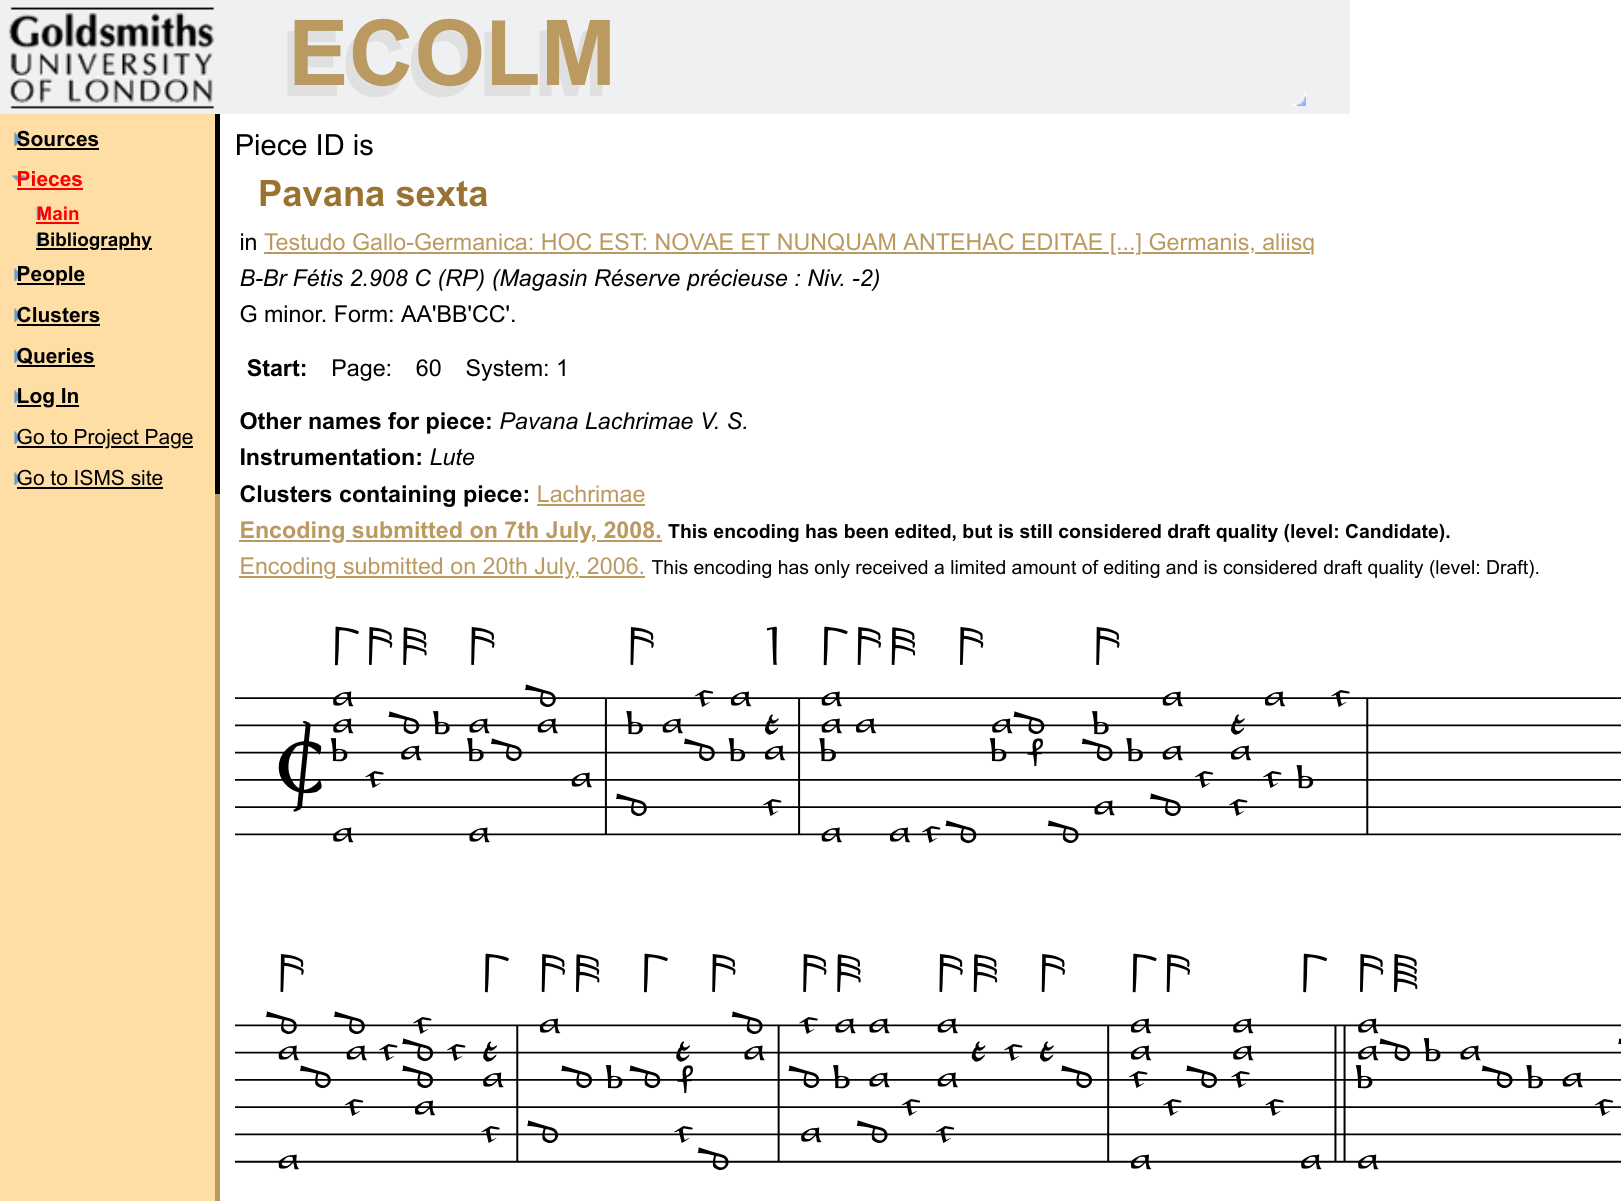
\includegraphics[width=0.9\columnwidth,frame]{images/ecolm-screenshot}\\
  {\small The ECOLM interface as it appears today.}
  \end{center}\vspace{1cm}

  \noindent ECOLM is just one of the lute tablature resources we are
  concerned with. Others include {\bf lutemusic.org} by Sarge Gerbode;
  {\bf mss.slweiss.de} by Peter Steur and the late Markus Lutz; {\bf
    Lute Society publications} curated by John Robinson; and {\bf
    editions by Pierre Phal\`ese} curated by Jan Burgers. All either
  CC licensed or offered by their maintainers as possible constituents
  of a future combined tablature resource.

  \vspace{2cm}
  \noindent\textbf{\LARGE The Challenge}\\

  \noindent The problems these resources face are highly typical:
  curation and maintenance by \textbf{individuals or small groups of
    enthusiasts}, in some cases of retirement age; maintenance in
  \textbf{limited periods of spare time}; data management using
  \textbf{ad-hoc methods} or private systems that are not accessible
  to third-party reproduction; \textbf{lack of data export} facilities
  or support for common \textbf{interchange formats}.

  \noindent Lute tablature faces further difficulties because it is
  such a specialised field. Wider digital solutions for music
  distribution and study typically do not handle it and its resources
  face significant risk of becoming inaccessible.

  %% At the same time, as an enthusiast-curated field of transcriptions
  %% of uneven provenance, it has much in common with more popular fields
  %% such as rock guitar transcription or music for community
  %% choirs---areas that have largely focused on performance but may
  %% increasingly want to support scholarly applications. Resources such
  %% as CPDL (Choral Public Domain
  %% Library), Ultimate
  %% Guitar, or ABC Tune
  %% Search are similar curated
  %% or crowd-sourced resources of music transcriptions with editorial
  %% variations and limited metadata.

  %% Any solutions found to support sustainability in this area have the
  %% potential to be informative for these other fields as well. The
  %% niche status of lute tablature poses a problem for its users, but
  %% the general quality of the technical and social issues around it may
  %% present a source of more general solutions.

  \columnbreak
  \noindent\textbf{\LARGE Audiences}\\

  \noindent These resources serve a spectrum of audiences from
  performer to musicologist. We are most concerned with sustainability
  for musicology and other academic purposes. We asked three exemplary
  users of online early-music resources---a \textbf{musicologist}, a
  \textbf{computational musicologist}, and a \textbf{lute
    teacher}---for their views about them so as to understand
  scholarly expectations.

  \noindent They highlighted the importance of \textbf{trust and
    provenance}, particularly knowing about the quality of
  transcription and level of editorial intervention in a
  resource. There was some consensus about \textbf{the value of simple
    search} with subsequent refinement, of a \textbf{cleanly-designed
    results} layout including inline incipits, and of \textbf{API and
    data provision}.

  \noindent Resources regarded as worth studying included DIAMM
  (Digital Image Archive of Medieval Music), the Vihuela Database, the
  Josquin Research Project, and RISM (R\'epertoire International des
  Sources Musicales) which is a near-ubiquitous entry point for
  musicological queries.

  \begin{center}\vspace{1cm}
    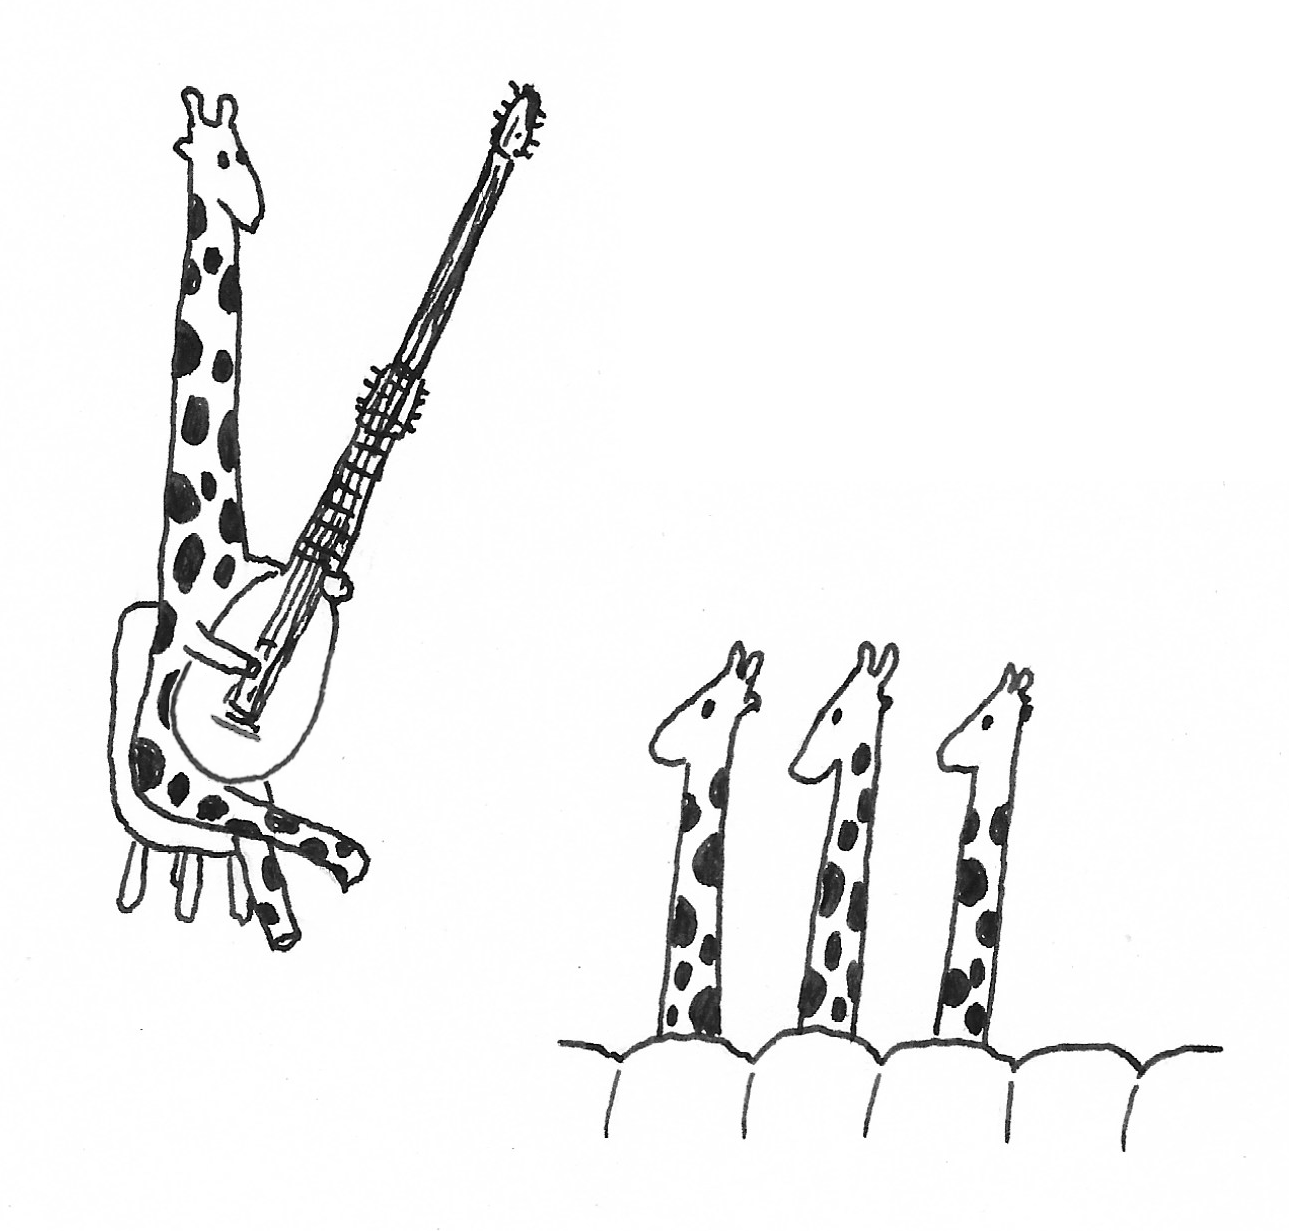
\includegraphics[width=0.7\columnwidth]{images/giraffe-archlute-2}\\
    \vspace{-1cm}
  {\small A giraffe playing an archlute.}
    \vspace{1cm}
  \end{center}

  \vspace{1cm}
  \noindent\textbf{\LARGE Possible Future Directions}\\
  \vspace{-2cm}
  \section{``Enhanced ECOLM''}

  Retain the relational data schema of ECOLM, the only one of the
  datasets to have a formal schema. Provide data loaders for other
  sources. Publish schema, data dumps, automation to rebuild or mirror
  the data, and the code of a query interface. Encourage others to
  add their own tools.

  \noindent\textbf{Advantages:} Ability to preserve existing code and
  use ECOLM as a reference. Schema has some good design
  decisions. Relational data import is well understood. Can focus on
  UI and data conversion. Relatively low-risk.

  \noindent\textbf{Disadvantages:} Schema has little in common with
  the other ad-hoc solutions, so all import and export would be
  custom. Also little in common with wider current practice. Does not
  solve problems relating to stable identifiers, versioning, or
  providing queryable APIs or data sources.

  \section{Graph-based}

  Take fundamental representation to be a graph of triples like
  RDF. Convert all metadata to that for import, and from it for
  query. Identify external data (transcriptions, media) by graph IDs
  such as URIs.

  \noindent\textbf{Advantages:} Widely-understood and accepted model
  meeting common expectations about compatibility and APIs. Can draw
  ontologies from existing systems. Reasonably amenable to versioning
  and to use of ``idempotent'' import flows with automated testing,
  for ongoing import of upstream changes. Could be more easily
  maintained or mirrored by third parties.

  \noindent\textbf{Disadvantages:} Requires all existing data to be
  converted and discards existing UI. Graphs not generally used for
  manual data management, so little in common with existing ad-hoc
  schemas of enthusiasts. Stable identifier mappings still hard. Good
  testing required to avoid ``silently missing data'' on query. Does
  not address non-graph data such as media.
  
  \section{``RISM-aligned''}

  Focus on compatibility with formats and software used by RISM as the
  dominant ``entry point'' in this field. Though our sources are not
  all up to the standard indexed by RISM, we want to facilitate
  linkage for those that are, and to be prepared if in the future RISM
  should grow to cover the whole area of directly represented lute
  tablature. The ideal future here would involve replacing this
  project entirely with an aspect of RISM.

  \noindent In this approach the metadata representation might be MARC
  (Machine Readable Cataloging) as it is within RISM, and possibly the
  RISM Muscat application might be used for management.

  \vspace{2cm}
  \noindent\textbf{\LARGE Summary}\\

  \noindent These three directions correspond to common patterns in
  work of this type:

  \begin{enumerate}
  \item Choose one of the existing technical solutions and adapt the
    others to it;
  \item Adopt a higher-level (``linked data'') approach in which
    existing resources are promoted to a common format;
  \item Find an industry partner, adopt their tools, and contribute to
    their existing ecosystem.
  \end{enumerate}
  
\end{sloppypar}
  
\end{multicols}
\end{document}
